\documentclass[french]{beamer}

\usepackage[frenchb]{babel}
\usepackage[T1]{fontenc}
\usepackage[utf8]{inputenc}
\usepackage{amsmath}
\usepackage{listings}

\usetheme{Hannover}

\begin{document}

\begin{frame}
	\tableofcontents
\end{frame}

\section{Complexite}

\begin{frame}
	En théorie :
	\begin{itemize}
		\item Opérations vectorielles : GPU. \;\;\;\;\; $\nu(n)$
		\item Autres : CPU.
	\end{itemize}
	En pratique :
	\begin{itemize}
		\item Opération vectorielles : numpy, boucles sous-jacentes en C.
		\item Autres : python
	\end{itemize}
	Objectif : Vectoriser au maximum les opérations.
\end{frame}

\section{LAB}

\begin{frame}
	\frametitle{LAB}
	\begin{columns}
		\begin{column}{5cm}
			$$L = \frac{R + G + B}{3}$$
			$$A = \frac{G - R + 255}{2}$$
			$$B = \frac{G - B + 255}{2}$$
		\end{column}
		\begin{column}{5cm}
			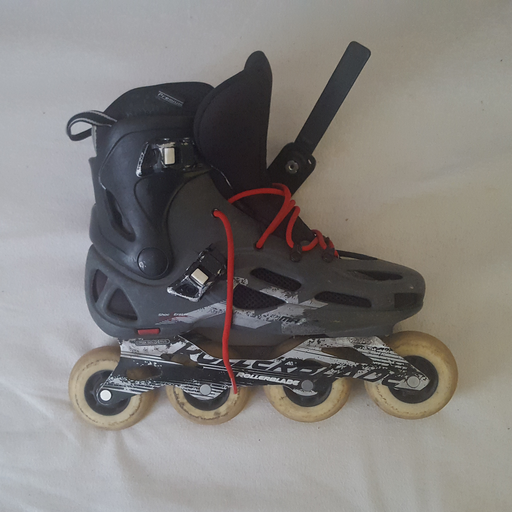
\includegraphics[width=3cm]{images/roller.png}\\
			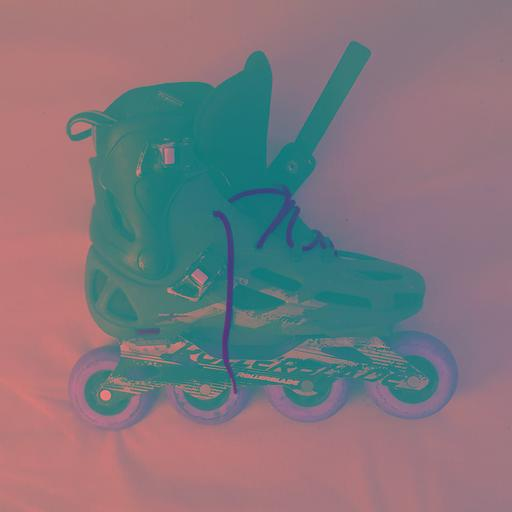
\includegraphics[width=3cm]{images/roller_lab.jpg}
		\end{column}
	\end{columns}
	Complexité : $\theta(\nu(h \cdot l))$
\end{frame}

\section{Texture}

\begin{frame}
	\frametitle{Transformée de Fourier}
	Définition :
	\begin{itemize}
		\item Continue :\; $F(f)(s) = \frac{1}{\sqrt{2\pi}} \int_a^b e^{- 2i\pi sx} \cdot f(x) \, \mathrm dx$ \\
		\item Discrete :\; $FD(u)(k) = \frac{1}{\sqrt{N}} \sum\limits_{n = 0}^{n = N - 1} e^{-2i\pi \frac{kn}{N}} \cdot u{n}$
	\end{itemize}
	Propriétés
	\begin{itemize}
		\item Involutive : $F(F(f)) = f$ \; $DF(DF(u)) = u$
		\item Symétrie : $u \text{réelle} \implies DF(u) \text{paire}$
		\item Convolution : $u \star v = DF(u) \cdot DF(v)$ (Au facteur près)
	\end{itemize}
	Complexité temporelle
	\begin{itemize}
		\item Sur un vecteur : $\theta(l \cdot \nu(l))$
		\item Sur une image : $\theta((h \cdot  l) (\nu(h) + \nu(l))$
	\end{itemize}
	Complexité spatiale : En place

\end{frame}

\begin{frame}[allowframebreaks]
	\frametitle{Transformée de Fourier rapide}
	Diviser pour régner\\
	Complexité temporelle
	\begin{itemize}
		\item Sur un vecteur : $\theta(\log_2(l)\nu(l))$
		\item Sur une image : $\theta(\log_2(h)\nu(l \cdot h) + \log_2(l)\nu(h \cdot l))$
	\end{itemize}
\end{frame}

\begin{frame}
	\frametitle{Exemples}
	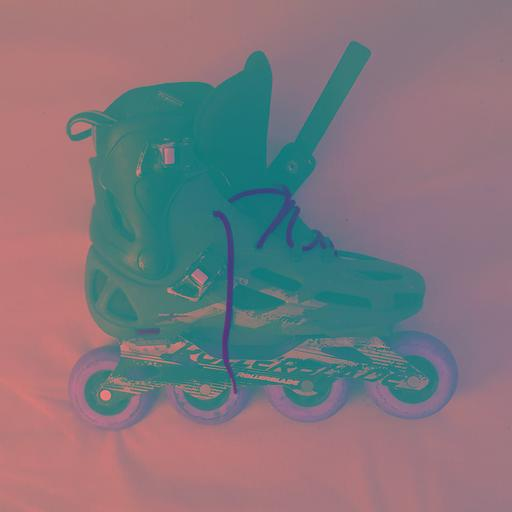
\includegraphics[width=3cm]{images/roller_lab.jpg} 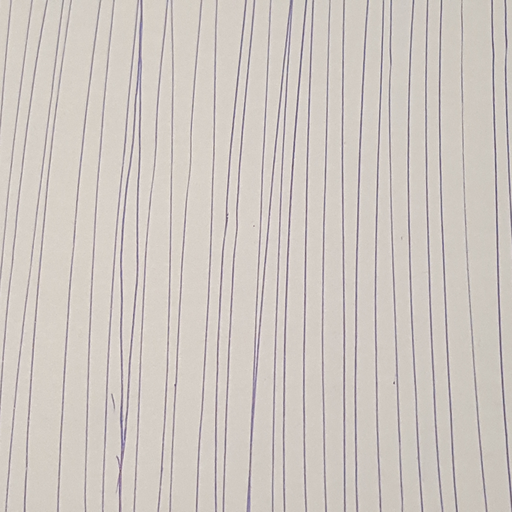
\includegraphics[width=3cm]{images/test1.png} 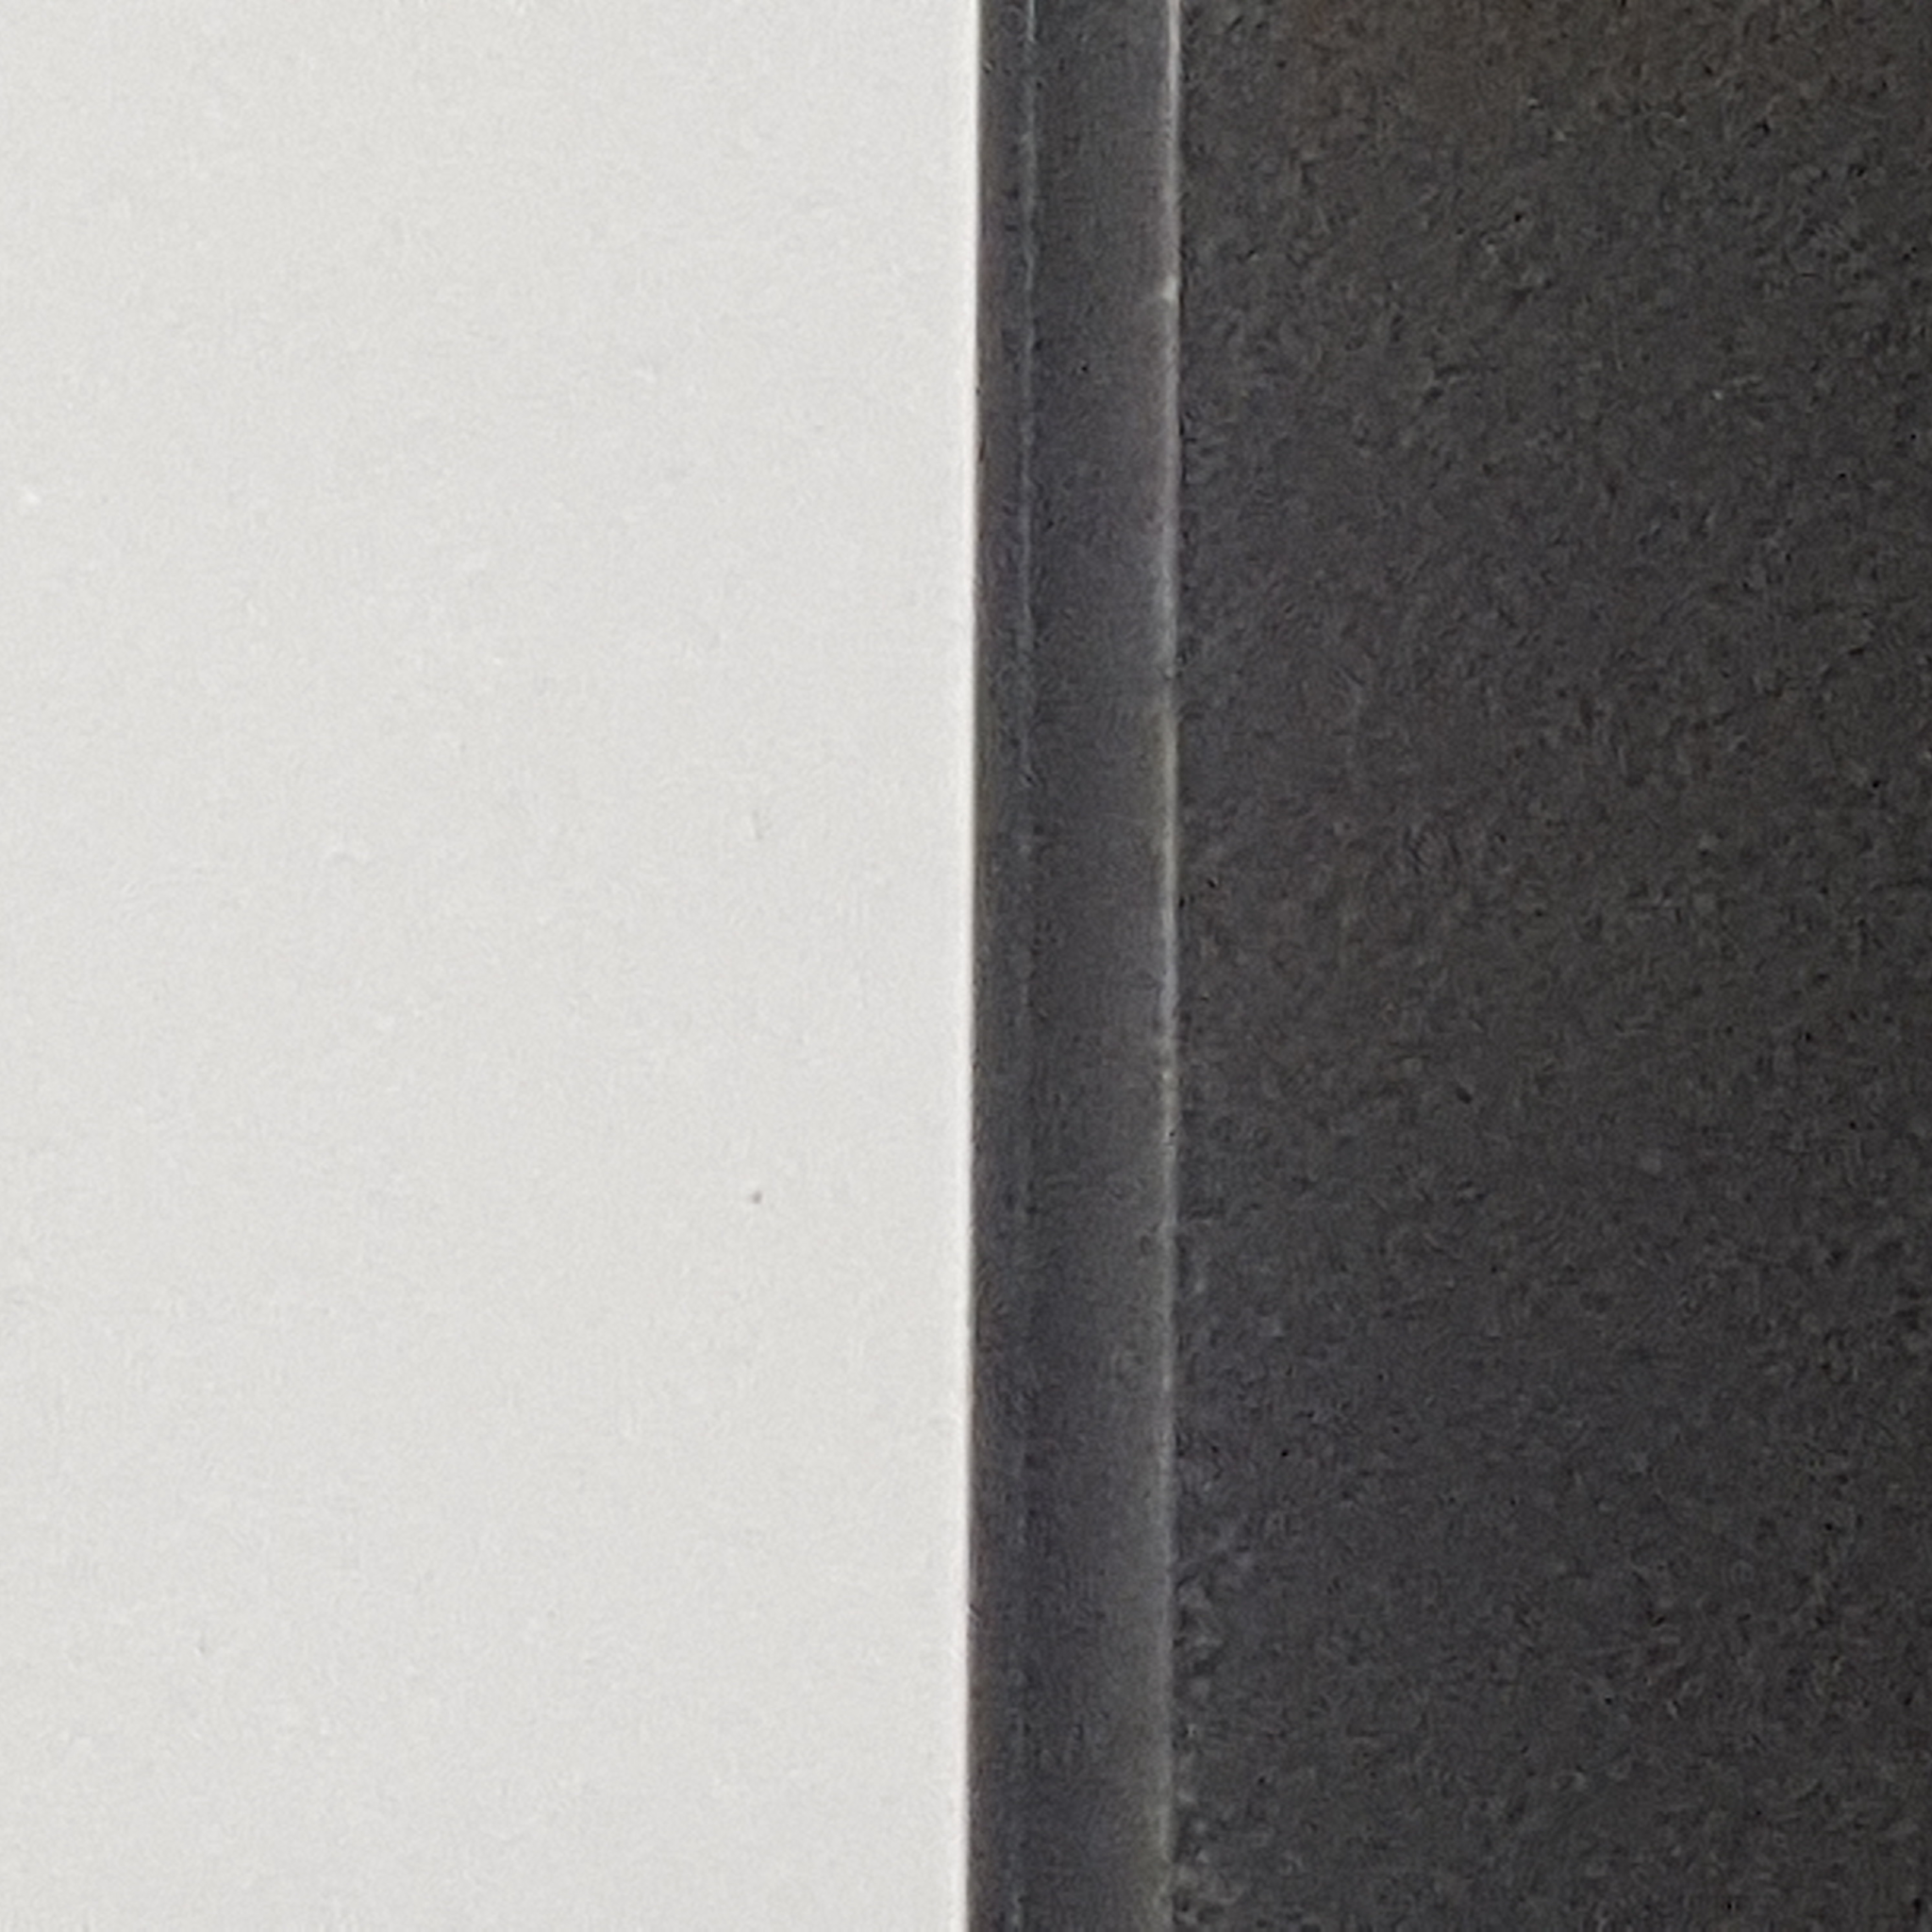
\includegraphics[width=3cm]{images/test2.png} \\ 
	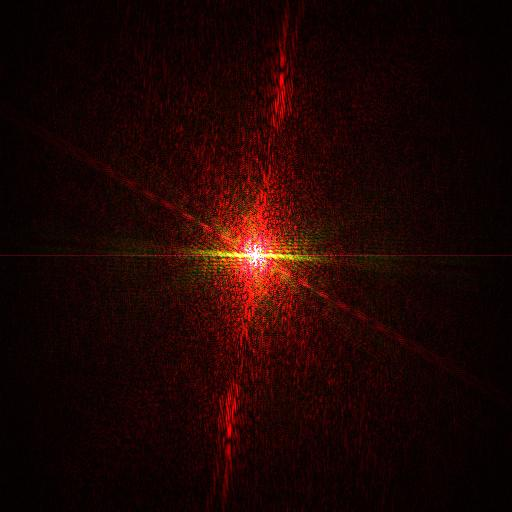
\includegraphics[width=3cm]{images/roller_fft.jpg} 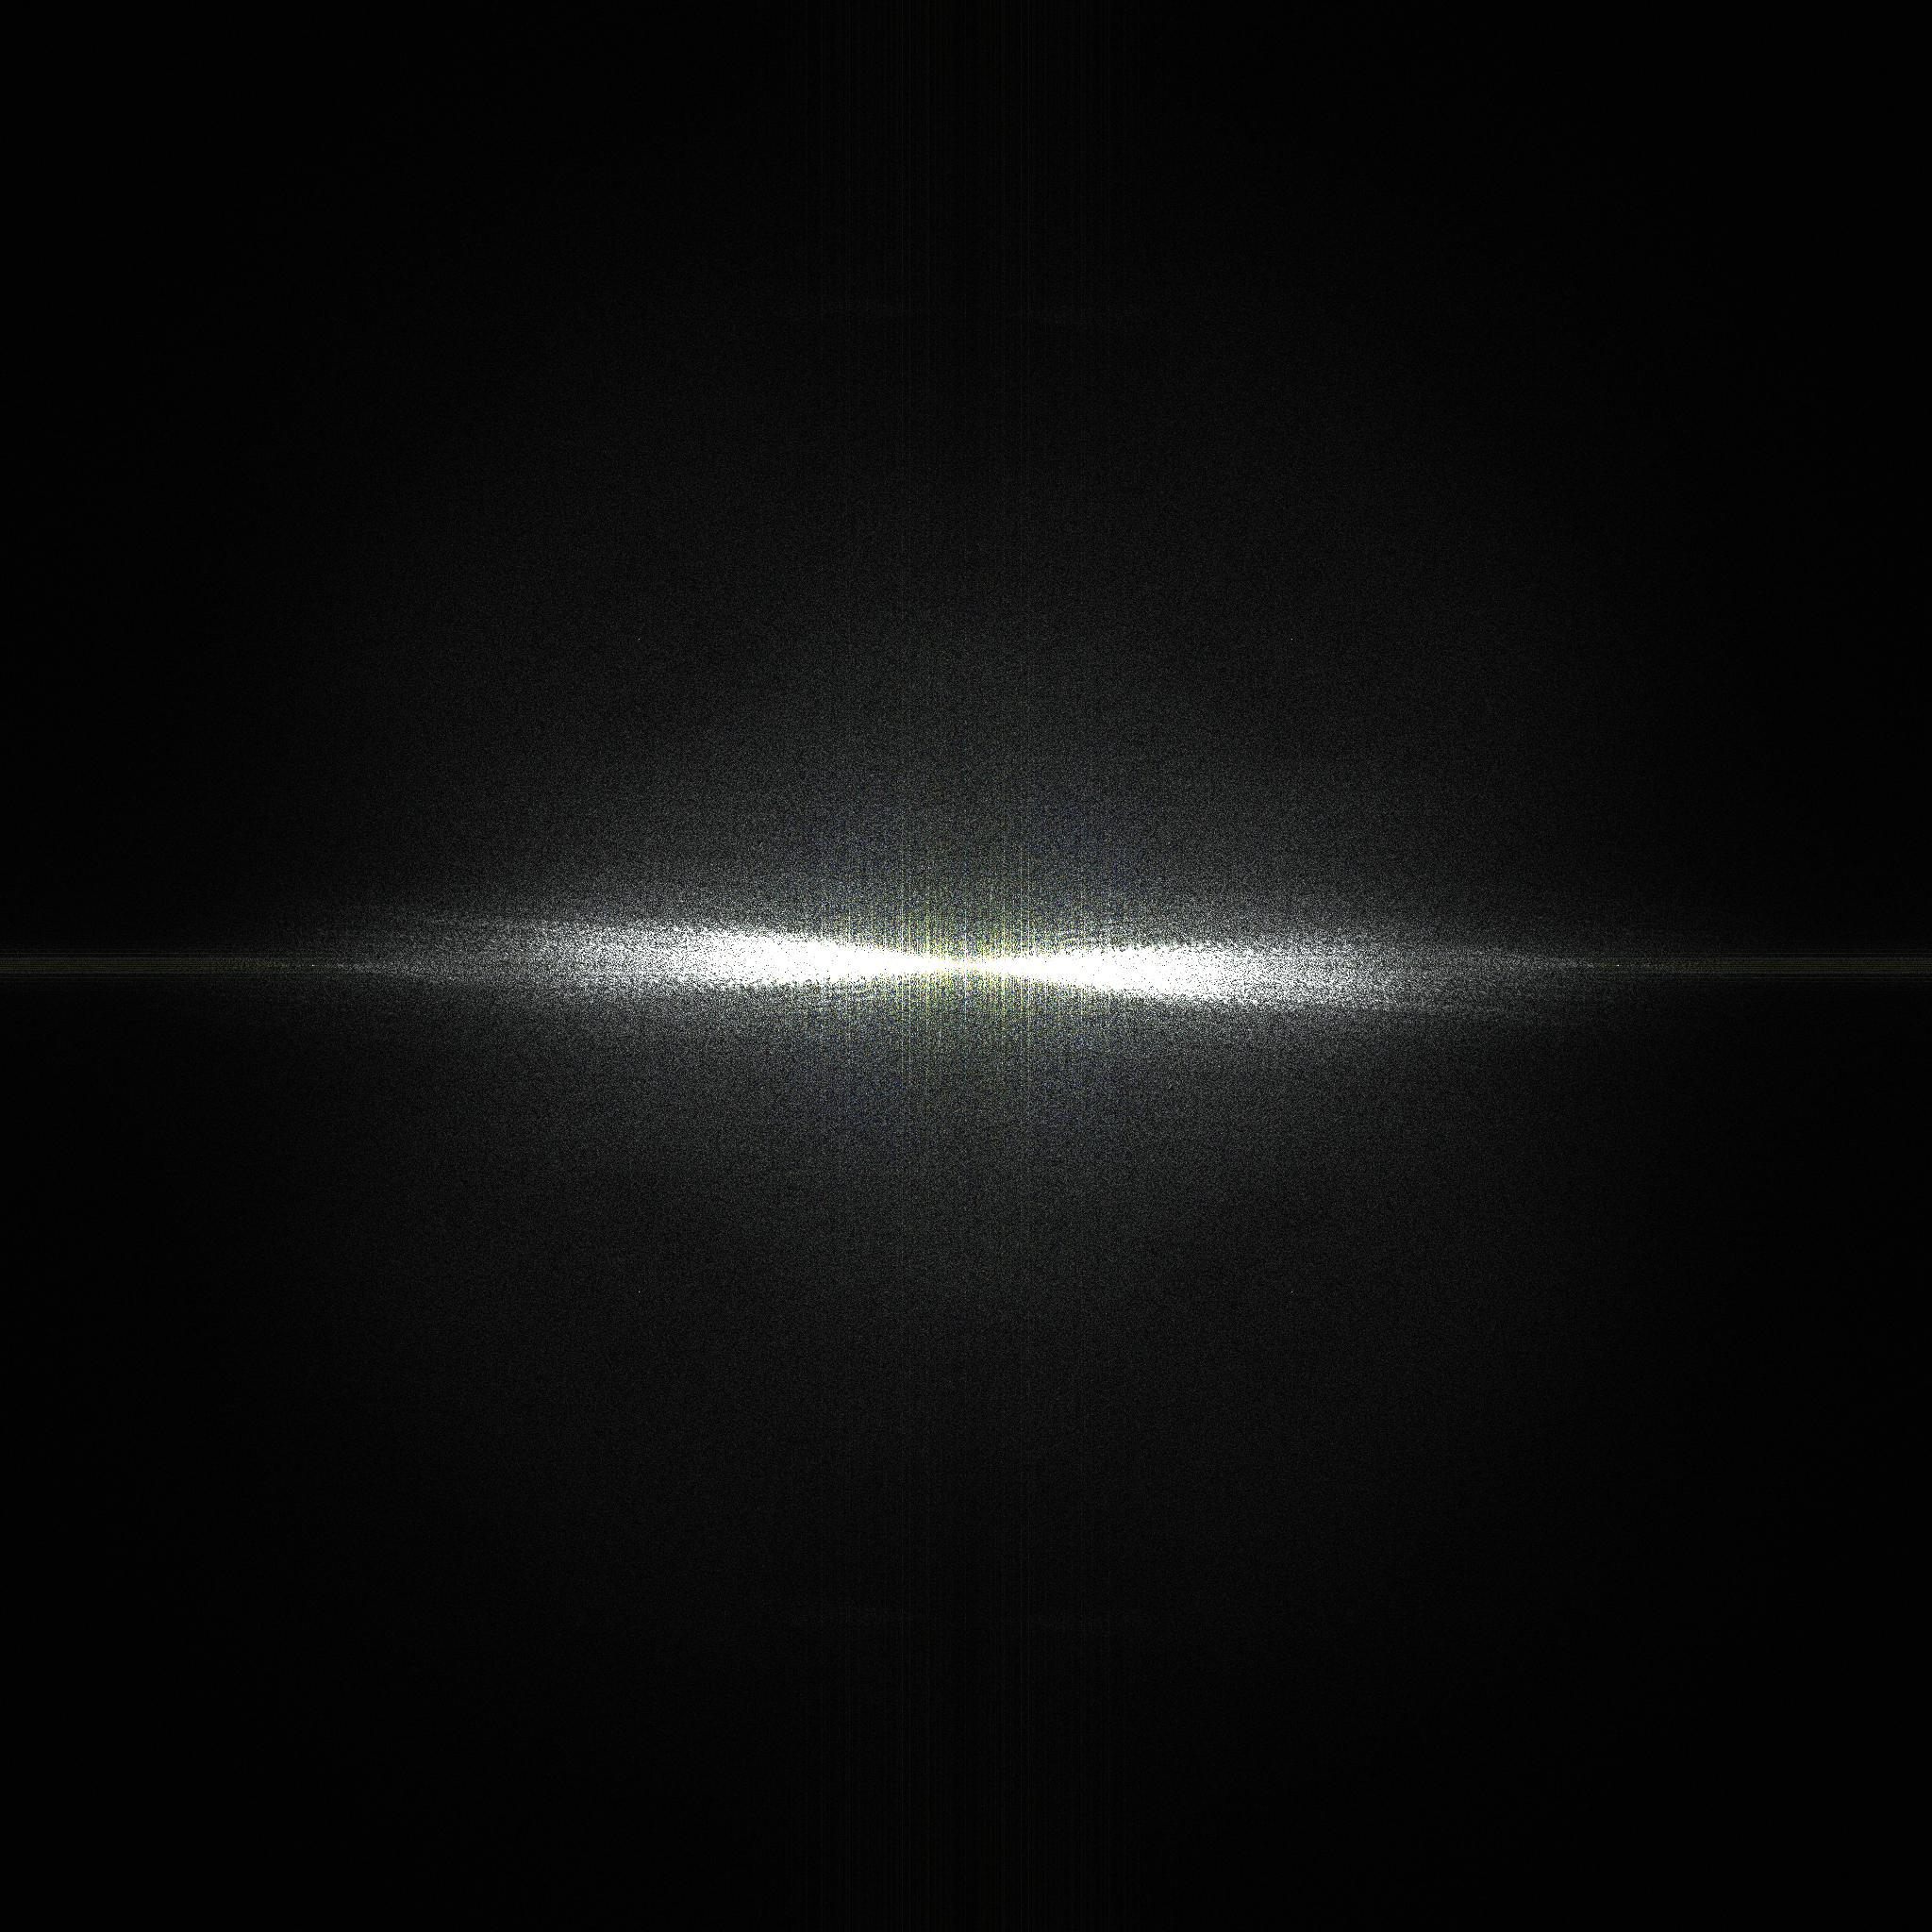
\includegraphics[width=3cm]{images/test1_fft.jpg} 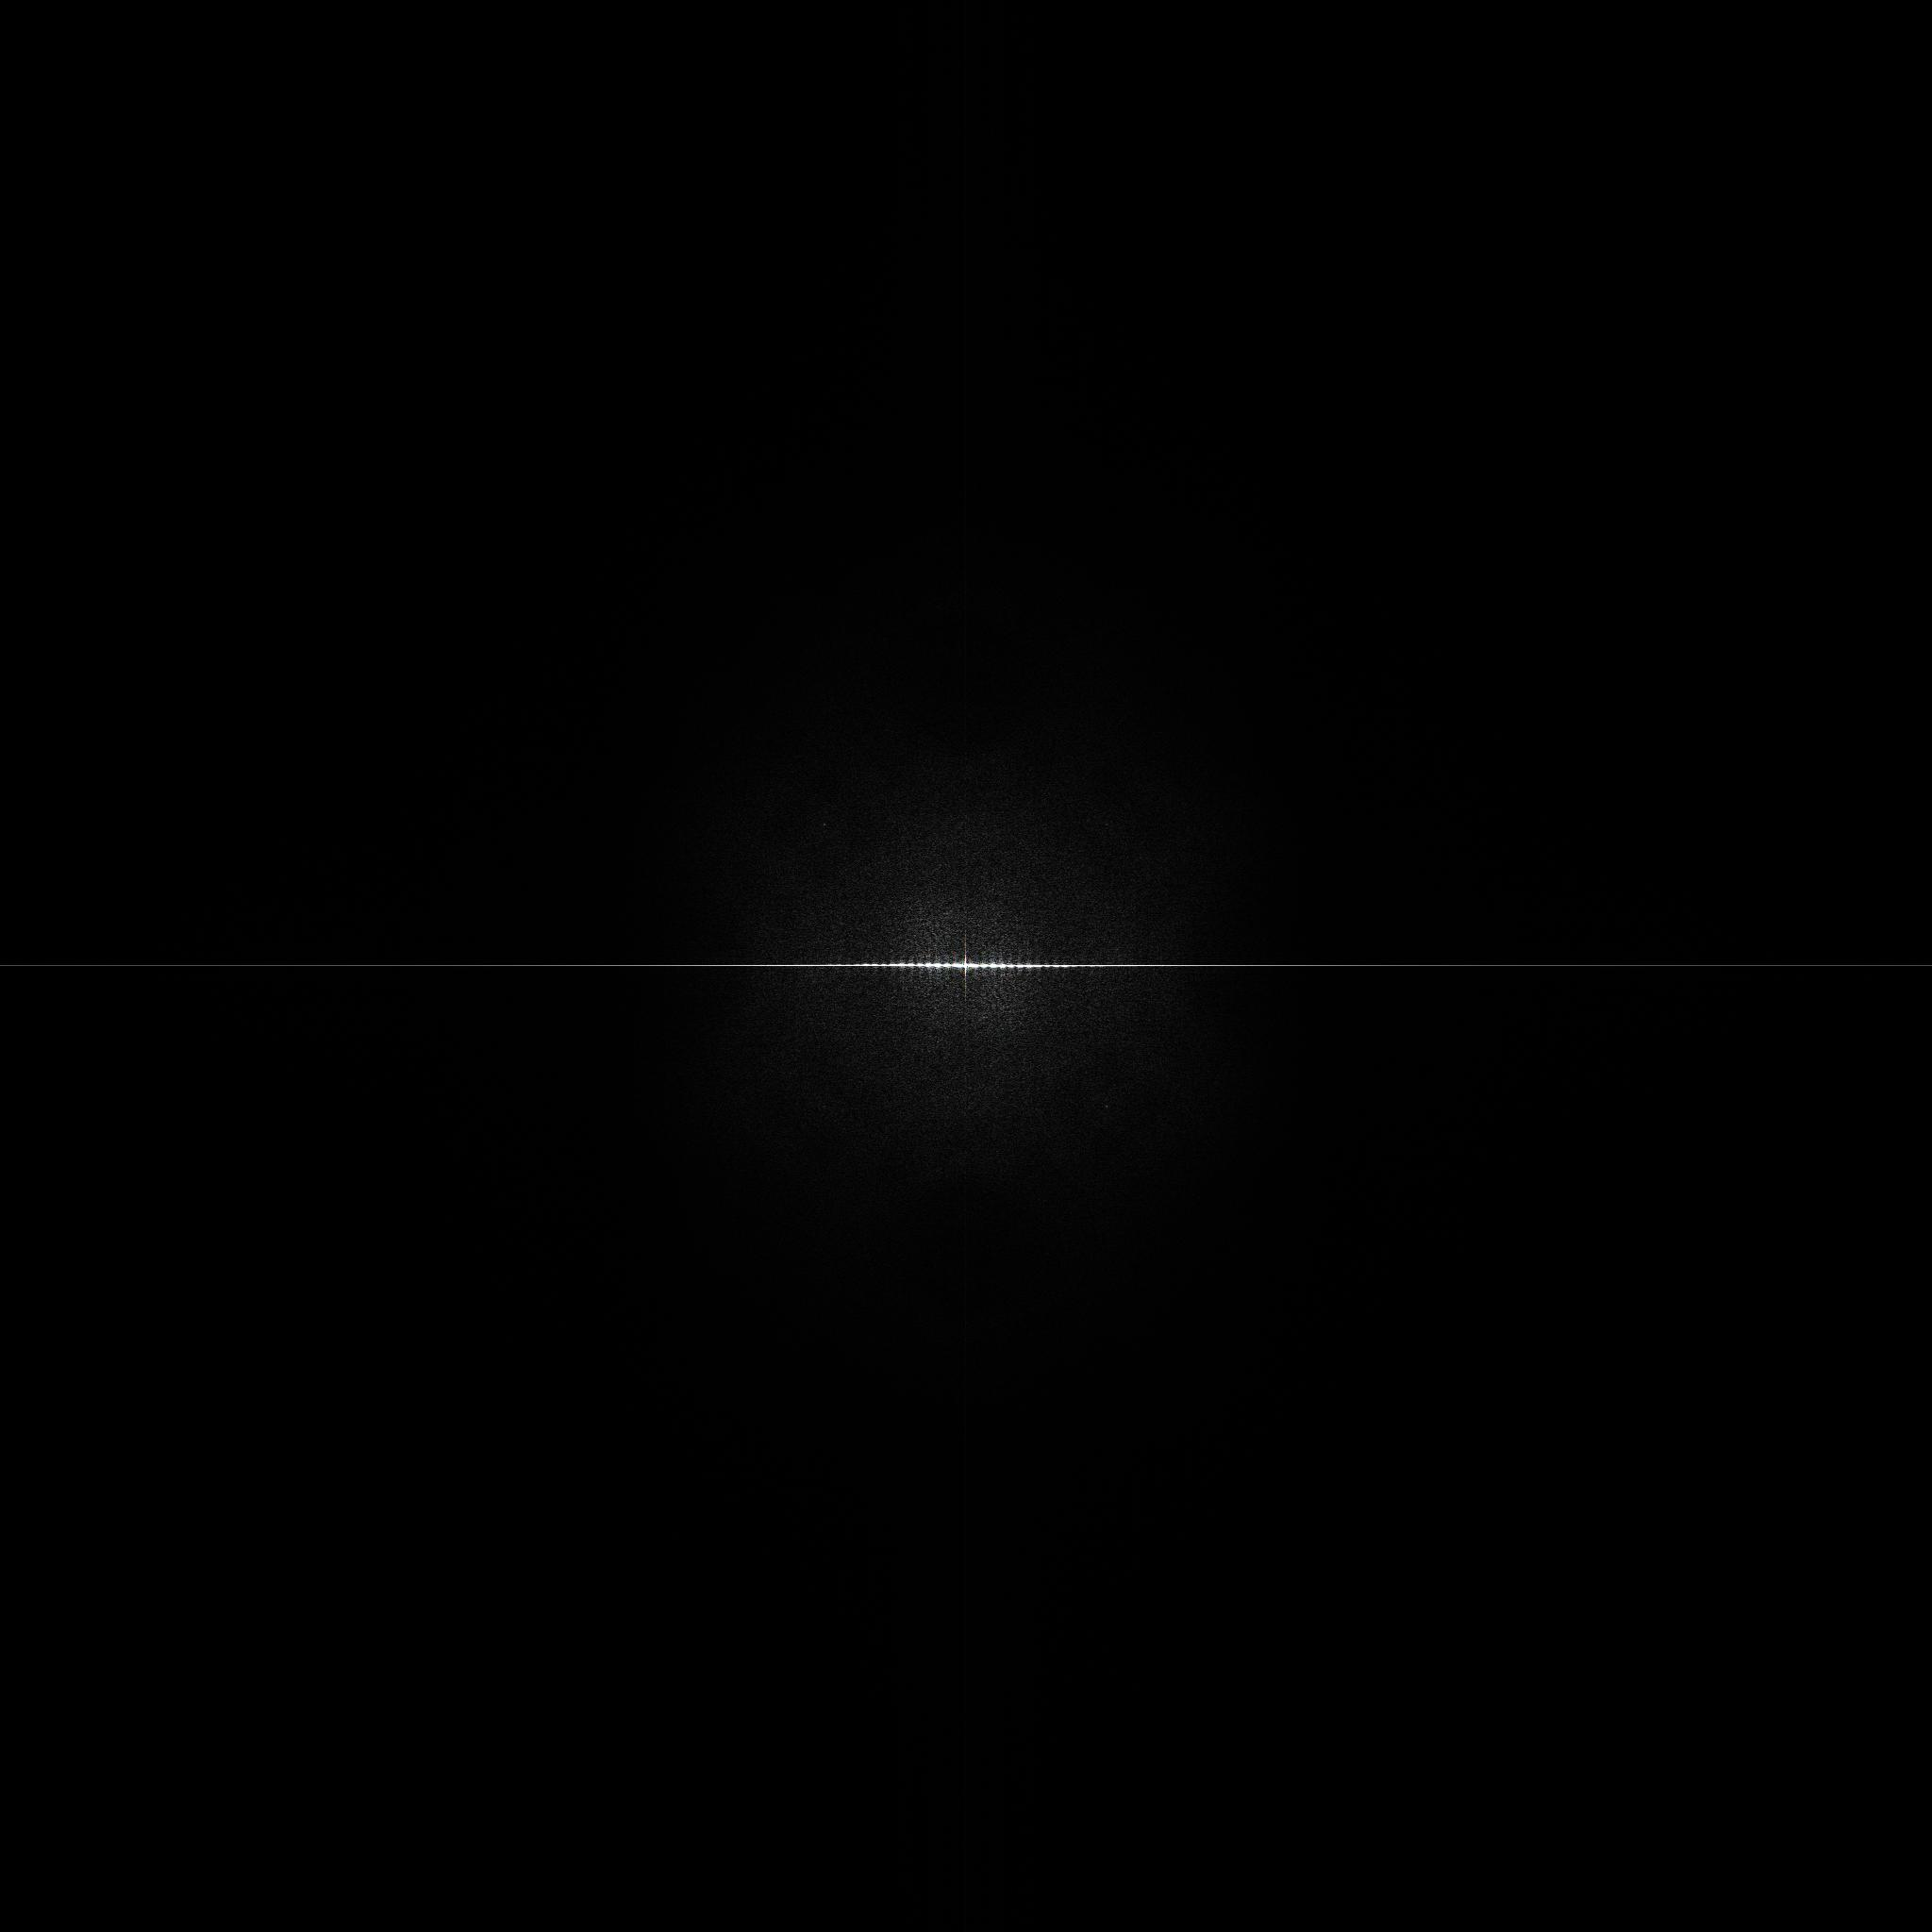
\includegraphics[width=3cm]{images/test2_fft.jpg}	
\end{frame}

\begin{frame}
	\frametitle{Filtres de convolution}
	\begin{columns}
		\begin{column}{5cm}
			Gaussienne d'orientation et d'écart type variable
			$$g(x) = e^{\frac{-x^2}{\sigma^2}}$$
		\end{column}
		\begin{column}{5cm}
			\begin{figure}[!h]
				\centering
				
\includegraphics[width=4cm]{images/fgauss.jpg}
				\caption{taille : 16, $\theta$ : $\frac{\pi}{6}$, $\sigma$ : 4}
			\end{figure}
		\end{column}
	\end{columns}
\end{frame}

\begin{frame}
	\frametitle{Exemples}
	\begin{figure}
		\centering
		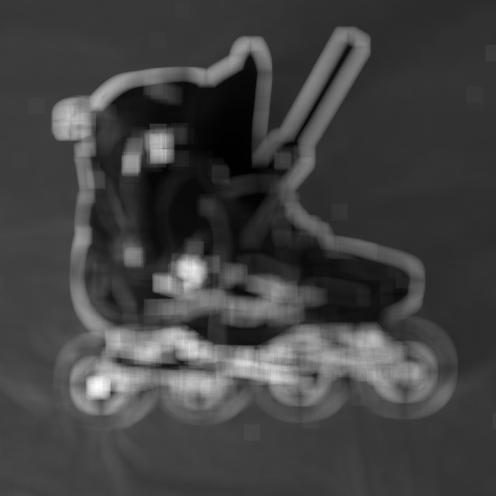
\includegraphics[width=5cm]{images/roller_resp.jpg}
		\caption{tailled : 16, $\theta$ : $\frac{\pi}{2}$, $\sigma$ : 4}
	\end{figure}
\end{frame}

\section{Filtrage}

\begin{frame}
	\frametitle{Procédé}
	\begin{itemize}
		\item Multiplication du voisinage de chaque pixel par le filter (centré sur le pixel)
		\item Sommation de toutes les valeures
	\end{itemize}
	En pratique : 
	\begin{itemize}
		\item On "décale" l'image de quelques pixels pour chaque coordonnée du filtre
		\item On multiplie chaque image décalée par le coefficient du filtre correspondant
		\item On ajoute les image ainsi obtenues
	\end{itemize}
	Complexité:
	\begin{itemize}
		\item Spatiale : En place
		\item Temporelle : $\theta(t^2 \cdot \nu(l \cdot h))$
	\end{itemize}
\end{frame}

\begin{frame}
	\frametitle{Filtre de Canny}
	\begin{columns}
		\begin{column}{5cm}
			Filtre optimal pour les aretes en "pas" 
			Dérivée d'une gaussienne:
			$$h(x) = x \cdot e^{-\frac{x^2}{\sigma^2}}$$
		\end{column}
		\begin{column}{5cm}
			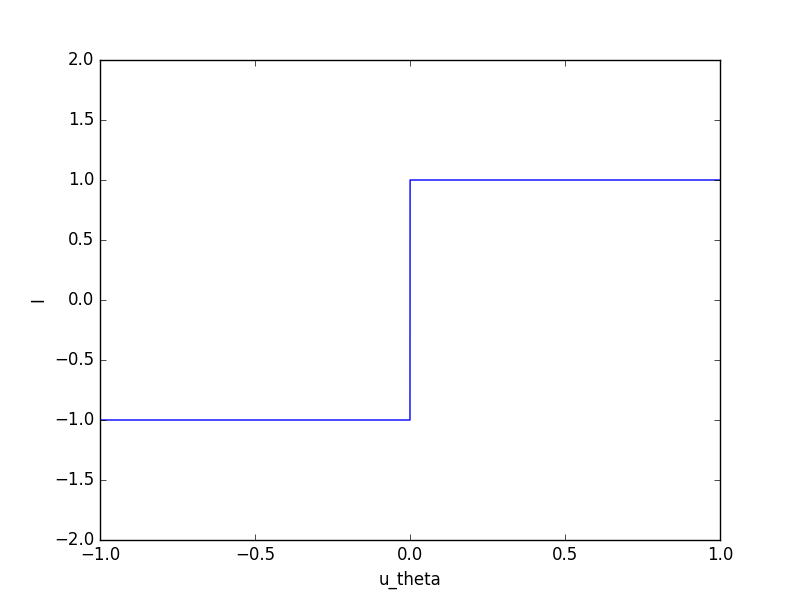
\includegraphics[width=3cm]{images/step.png}\\
			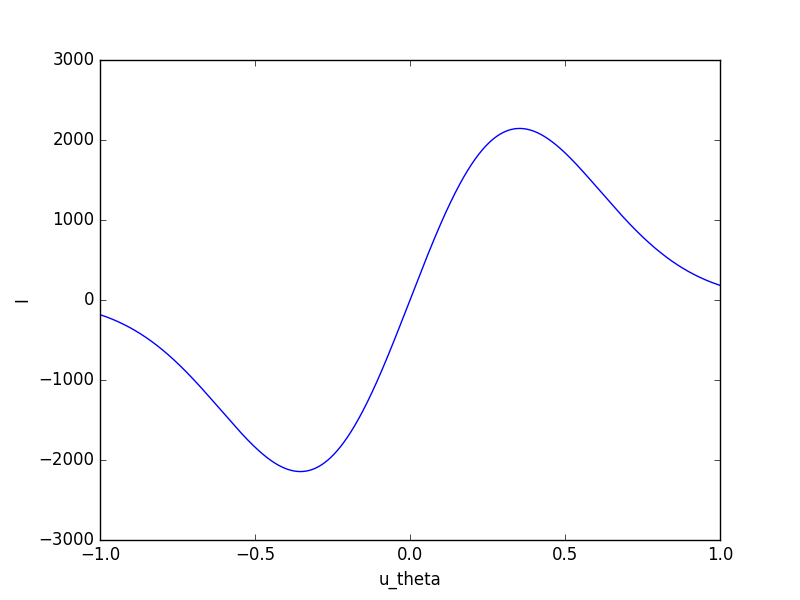
\includegraphics[width=3cm]{images/gaussd1d.png}\\
			
\includegraphics[width=3cm]{images/gaussd.png}
		\end{column}
	\end{columns}
\end{frame}

\begin{frame}
	\frametitle{Exemples}
	\begin{figure}[!h]
		\centering
		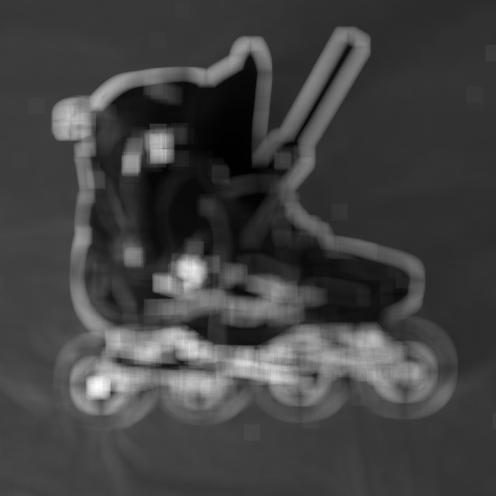
\includegraphics[width=4cm]{images/roller_resp.jpg} \; 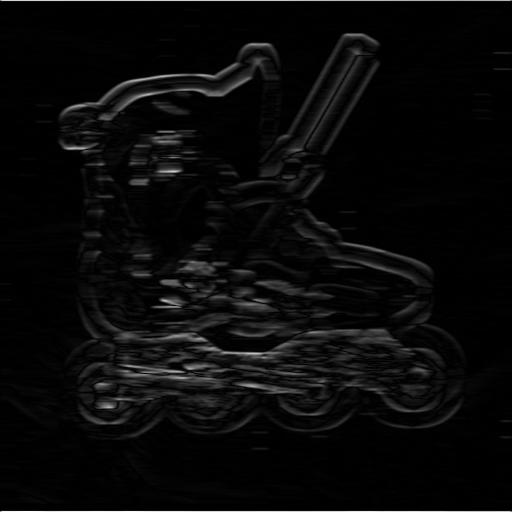
\includegraphics[width = 4cm]{images/roller_filtered.jpg}
		\caption{$\theta$ : $\frac{pi}{2}$, $\sigma$ : 1}
	\end{figure}
\end{frame}

\section{Localisation}

\begin{frame}
	\begin{columns}
		\begin{column}{5cm}
			Complexité Temporelle
			\begin{itemize}
				\item Projection : $\theta(\nu(t^2))$
				\item Approximation parabolique :
					\begin{itemize}
						\item Calcul des sommes : $\theta(t^2 \cdot \nu(h \cdot l))$
						\item Résolution des systèmes : $\theta(\nu(h \cdot l))$
					\end{itemize}
				\item Localisation : $\theta(\nu(h \cdot l))$
				\item Total temporel : $\theta(\nu(h \cdot l))$
			\end{itemize}
			Complexité spatiale : $\theta(t^2 \cdot h \cdot l)$
		\end{column}
		\begin{column}{5cm}
			\begin{figure}[!h]
				\includegraphics[width=4cm]{images/projection.jpeg}
				\caption{Projection}
			\end{figure}
			Approximation parabolique : $ax^2 + bx + c = 0$\\
			Localisation: $\hat{f}(x) = c^+ \cdot \frac{2a^-}{|b|}$
		\end{column}
	\end{columns}
\end{frame}

\begin{frame}
	\frametitle{Exemple}
	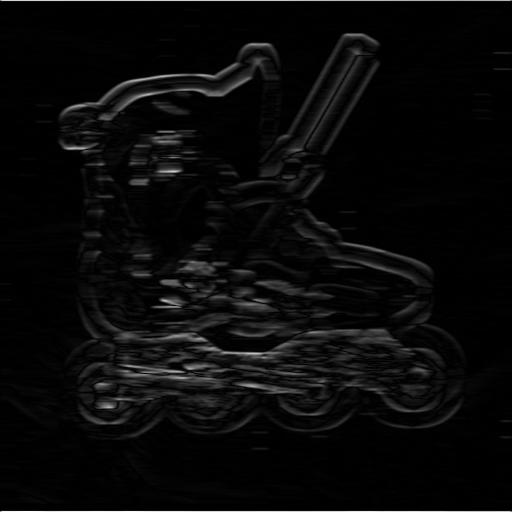
\includegraphics[width=4cm]{images/roller_filtered.jpg} \; 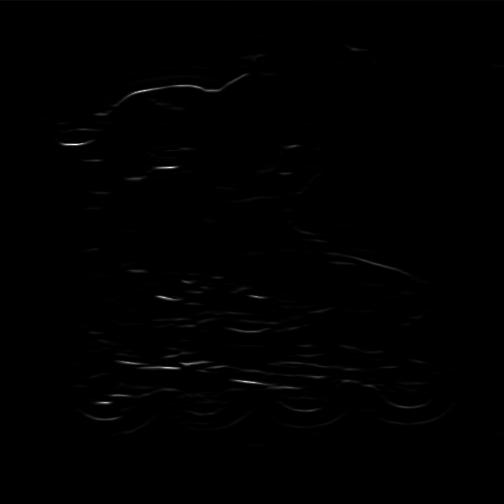
\includegraphics[width=4cm]{images/roller_localised.jpg}
\end{frame}

\section{Sommation des reponses}

\begin{frame}
	30 composantes:
	\begin{itemize}
		\item 3 couleurs + 3 couleurs * 4 directions = 15 composantes avant filtrage
		\item pour chaque composante, filtrage par deux filtres de Canny d'écart type 1 et 2 = 30 composantes
	\end{itemize}
	Choix des coefficients de sommation ?\\
	Approche optimale : apprentissage supervisé\\
	Ici : choix empirique
\end{frame}

\begin{frame}
	\frametitle{Exemple}
	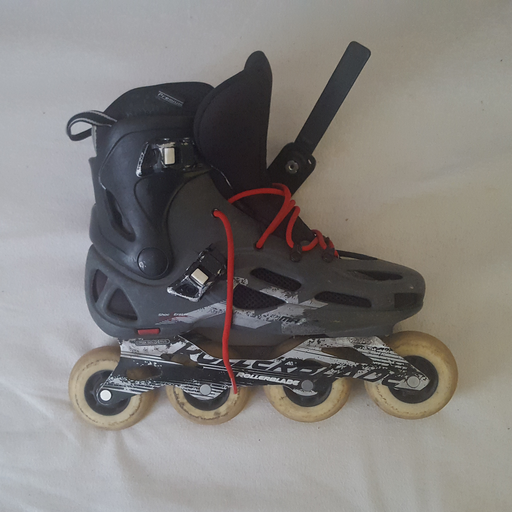
\includegraphics[width=4cm]{images/roller.png} \; 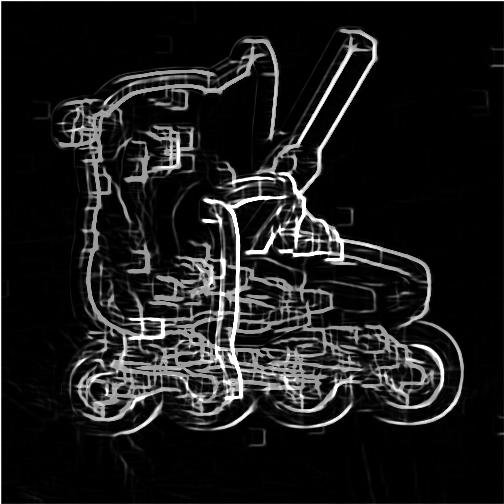
\includegraphics[width = 4cm]{images/roller_res.jpg}
\end{frame}

\section{Seuillage}

\begin{frame}
	Conversion en image binaire par seuillage:\\
	1 si I > seuil\\
	0 sinon\\
	\bigskip
	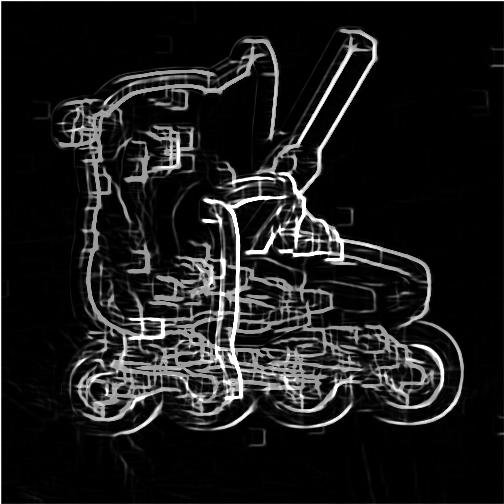
\includegraphics[width=3cm]{images/roller_res.jpg} \; 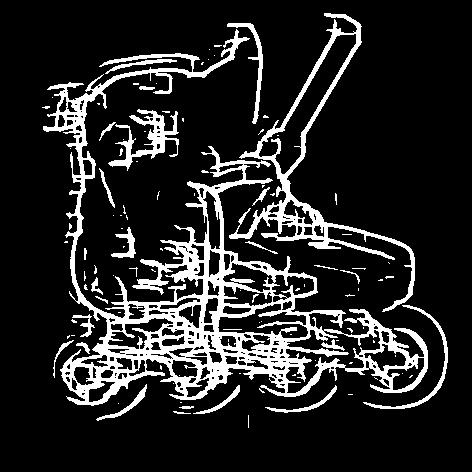
\includegraphics[width=3cm]{images/roller_bin.jpg}
\end{frame}

\section{Opérations topologiques}

\begin{frame}
	\frametitle{Définition}
	Même procédé de filtrage mais sur des images binaires
	\begin{columns}[T]
		\begin{column}{3cm}
			Erosion \\
			\bigskip
			\begin{tabular}{|l|c|r|}
				\hline
				0 & 1 & 0 \\ \hline
				1 & 1 & 1 \\ \hline
				0 & 1 & 0 \\
				\hline
			\end{tabular}
			\begin{tabular}{|l|c|c|c|r|}
				\hline
				0 & 0 & 0 & 0 & 0 \\ \hline
				0 & 1 & 0 & 1 & 0 \\ \hline
				0 & 1 & 1 & 1 & 0 \\ \hline
				1 & 1 & 1 & 1 & 1 \\ \hline
				1 & 1 & 1 & 1 & 1 \\
				\hline
			\end{tabular}
			\begin{tabular}{|l|c|c|c|r|}
				\hline
				0 & 0 & 0 & 0 & 0 \\ \hline
				0 & 0 & 1 & 1 & 0 \\ \hline
				0 & 1 & 1 & 1 & 0 \\ \hline
				0 & 0 & 1 & 1 & 1 \\ \hline
				0 & 0 & 1 & 1 & 1 \\
				\hline
			\end{tabular}
		\end{column}
		\begin{column}{3cm}
			Dilatation \\
			\bigskip
			\begin{tabular}{|l|c|r|}
				\hline
				0 & 0 & 0 \\ \hline
				1 & 1 & 1 \\ \hline
				0 & 0 & 0 \\
				\hline
			\end{tabular}
			\begin{tabular}{|l|c|c|c|r|}
				\hline
				0 & 0 & 0 & 0 & 0 \\ \hline
				0 & 1 & 1 & 1 & 0 \\ \hline
				0 & 0 & 0 & 0 & 1 \\ \hline
				1 & 1 & 1 & 1 & 1 \\ \hline
				1 & 1 & 1 & 1 & 1 \\
				\hline
			\end{tabular}
			\begin{tabular}{|l|c|c|c|r|}
				\hline
				0 & 0 & 0 & 0 & 0 \\ \hline
				0 & 0 & 0 & 0 & 0 \\ \hline
				1 & 1 & 0 & 0 & 0 \\ \hline
				0 & 0 & 0 & 0 & 0 \\ \hline
				0 & 0 & 0 & 0 & 0 \\
				\hline
			\end{tabular}
		\end{column}
		\begin{column}{3cm}
			Fermeture \\
			\bigskip
			Dilatation + Erosion
		\end{column}
	\end{columns}
\end{frame}

\begin{frame}
	\begin{columns}
		\begin{column}{5cm}
			\frametitle{Exemples}
			Erosion par : \\
			\medskip
			\begin{tabular}{|l|c|r|}
				\hline
				0 & 1 & 0 \\ \hline
				1 & 1 & 1 \\ \hline
				0 & 1 & 0 \\
				\hline
			\end{tabular} \\
			\medskip
			Fermeture par : \\
			\medskip
			\begin{tabular}{|l|c|c|c|r|}
				\hline
				0 & 0 & 0 & 0 & 0 \\ \hline
				0 & 0 & 0 & 0 & 0 \\ \hline
				1 & 1 & 1 & 1 & 1 \\ \hline
				0 & 0 & 0 & 0 & 0 \\ \hline
				0 & 0 & 0 & 0 & 0 \\
				\hline
			\end{tabular} \\
			\medskip
			Auquel on applique des rotations dans 8 directions différentes
		\end{column}
		\begin{column}{5cm}
			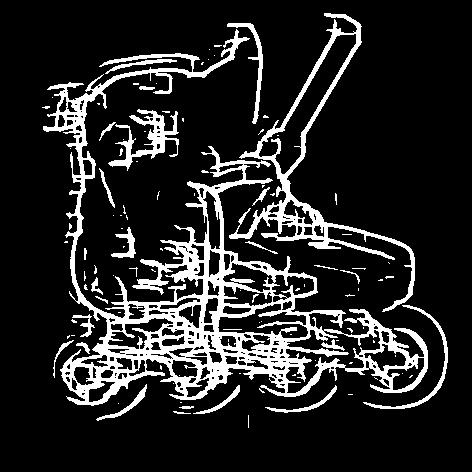
\includegraphics[width=2cm]{images/roller_bin.jpg}\\
			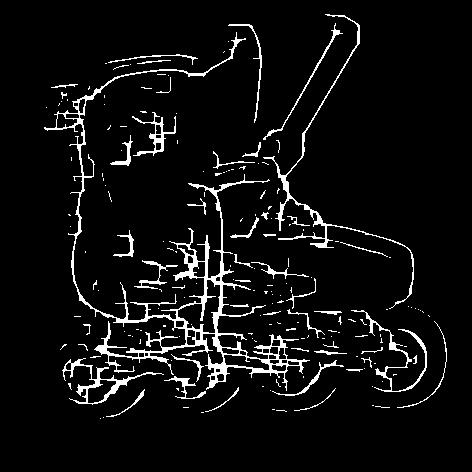
\includegraphics[width=2cm]{images/roller_bin-.jpg}\\
			
\includegraphics[width=2cm]{images/roller_closedbin.jpg}
		\end{column}
	\end{columns}
\end{frame}

\section{Contours}

\begin{frame}
	\frametitle{Parcours du contour}
	Parcours dans le sens trigonométrique\\
	Départ du pixel le plus en haut\\
	Direction initiale : Bas \\
	Priorités de déplacement : Gauche - Bas - Droite - Haut\\
	\bigskip
	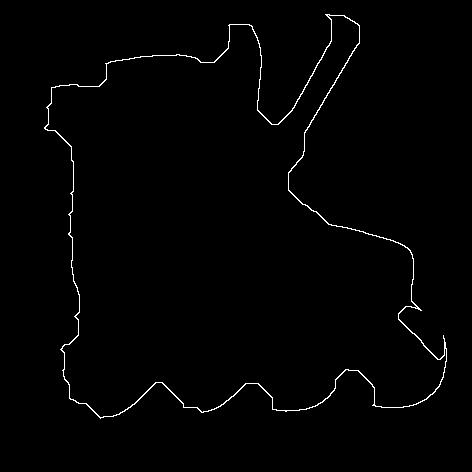
\includegraphics[width=5cm]{images/roller_contour.jpg}
\end{frame}

\begin{frame}
	\frametitle{Approximation affine}
	Initialisation : Point le plus haut - Point le plus bas\\
	Sur chaque segment, successivement :
	\begin{itemize}
		\item Calcul de $D$ distance max du contour au segment
		\item Si $D > \text{seuil}$, on ajoute le point le plus éloigné
		\item Lorsque pour tout segment $D < \text{seuil}$, on sort de la boucle
	\end{itemize}
\end{frame}

\section{Annexe}

\begin{frame}[allowframebreaks]
	\frametitle{Transformée de Fourier rapide}
	Notation :
	\begin{itemize}
		\item $N = 2p$
		\item $n = n_1 + pn_2 \;\;\;\;\; n_1 \in (0, p-1) \;\;\; n_2 \in {0, 1}$
		\item $k = 2k_1 + k_2 \;\;\;\;\; k_1 \in (0, p-1) \;\;\; k_2 \in {0, 1}$
		\item $a = e^{-\frac{2i\pi}{N}}$
	\end{itemize}
	Alors :
	\begin{eqnarray}
		F(u)(k) & = & \sum\limits_{n = 0}^{N-1} u(n) \cdot a^{kn} \\
		F(u)(2k_1 + k_2) & = & \sum\limits_{n_1 = 0}^{1} \sum\limits_{n_2 = 0}^{p-1} u(n_1 + pn_2) \cdot a^{k \cdot (n_1 + pn_2)} \\
		& = & \sum\limits_{n_1 = 0}^{1} \sum\limits_{n_2 = 0}^{p-1} u(n_1 + pn_2) \cdot a^{kn_1} \cdot a^{kpn_2}
	\end{eqnarray}
	De plus :
	$a^{kpn_2} = a^{2p \cdot k_1n_2} \cdot a^{k_2n_1p} = a^{k_2n_1p}$ \\
	Ainsi :
	$F(u)(2k_1 + k_2) = \sum\limits_{n_1 = 0}^{1} a^{kn_1} \cdot \sum\limits_{n_2 = 0}^{p-1} u(n_1 + pn_2) \cdot a^{k_2n_1p}$ \\
	Posons :
	$ v(n_1, k_2) = \sum\limits_{n_2 = 0}^{p-1} u(n_1 + pn_2) \cdot a^{k_2n_1p}$ \\
	Finalement: 
	$F(u)(2k_1 + k_2) = v(0, k_2) + a^{k} \cdot v(1, k_2)$\\
	Le calcul de $v$ est celui d'une transformée de Fourier discrète. On applique récursivement la décomposition
	\bigskip
\end{frame}

\end{document}
